\subsubsection{Fine-tuning from \mfourttwo}
Most existing frameworks in streaming translation require training the model from scratch.
These approaches often require substantial resources, 
especially in large multilingual scenarios, such as \mfourttwo.
To leverage the language coverage and semantics accuracy achieved with the foundational \mfourttwo model,
we introduced a two-stage scheme for streaming fine-tuning, as shown in \Cref{fig:streaming.finetuning}.
\begin{figure}[!ht]
    \centering
    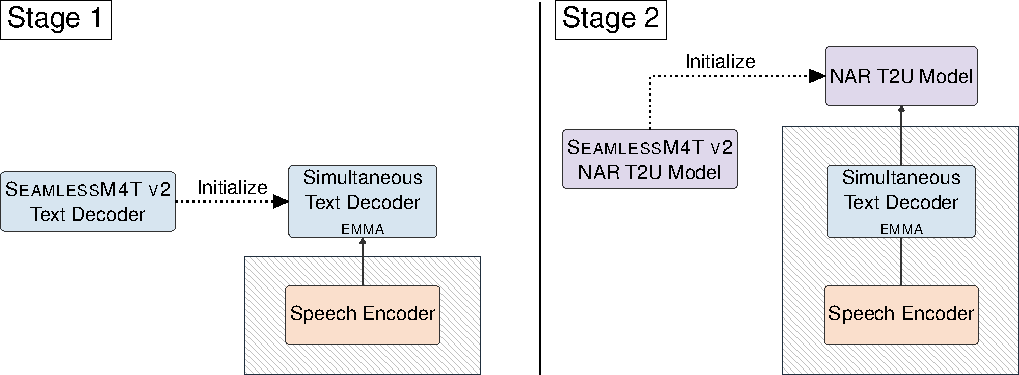
\includegraphics[width=0.8\textwidth]{figures/streaming/finetune.pdf}
    \caption{Streaming Finetuning of \seamlessstreaming from \mfourttwo. The weight of the module in shadowed boxes were frozen during training.}
    \label{fig:streaming.finetuning}
\end{figure}

In the first stage, 
we only trained a simultaneous speech-to-text model.
For the encoder, we reused the \mfourttwo speech encoder and froze it during training.
For the decoder, we initialized the parameters of generation network from \mfourttwo text decoder, 
and randomly initialize stepwise probability networks.
Furthermore, we added a negitive bias to the stepwise probability networks to let policy optimize from offline policy.

In the second stage, 
we froze the speech-to-text part of the model,
and only trained the text-to-unit model.
Similar to the text decoder,
we initialized the text-to-unit model from \mfourttwo. 

For streaming-finetuning, we only used the label and pseudo-labled data described in \Cref{sec:offline:data}.

\subsubsection{Streaming inference}
\label{sec:streaming.inference}
We used \simuleval \citep{ma_simuleval_2020} to build the streaming inference pipeline.
The overall inference algorithm is illustrated in \Cref{algo:streaming.inference}.
For streaming speech input, we updated the whole encoder every time a new speech chunk is received by the model.
Then, we ran the text decoder to generate partial text translation based on a policy.
Finally, we passed the text output and decoder states to the text-to-unit model.
Because of the new non-autoregressive design of \unitytwo text-to-unit decoder (\Cref{sec:offline:unity2}),
we were able to directly feed text decoder states to text-to-unit model to generate aligned unit chunks
We only synthsized speech when the length of unit chunks were greater than a minimal number $L_{\text{unit}}$.
\algnewcommand\algorithmicinput{\textbf{Input:}}
\algnewcommand\algorithmicoutput{\textbf{Output:}}
\algnewcommand\Input{\item[\algorithmicinput]}%
\algnewcommand\Output{\item[\algorithmicoutput]}%
\begin{algorithm}[!tbh]
\small
  \caption{\seamlessstreaming Inference Algorithm}
  \label{algo:streaming.inference}
  \begin{algorithmic}[1]
    \Require{$\tgttext_{\text{lang}}$: Target language tag}
    \Require{$t_{\text{EMMA}}$ : Decision threshold for EMMA}
    \Require{$L_{\text{unit}}$: Minimal chunk size for units}
    \item[]
    \Input{Streaming speech $\srcspeech$}
    \Output{Streaming speech $\tgtspeech$}
    \Output{Streaming text $\tgttext$}
    \item[]
    \State $i \gets 1$, $j \gets 0$, $k \gets 0$, $\tgttext_0 \gets \tgttext_{\text{lang}}$
    \State $s_0 \gets \texttt{TextDecoder}(\tgttext_{0})$
    \While{$\tgttext_{i-1} \neq \texttt{EndOfSequence}$}
        \State $j \gets j + 1$
        \State $h_{\leq j} \gets \texttt{SpeechEncoder}(\srcspeech_{\leq j})$
 
  
        \While{$\tgttext_{i-1} \neq \texttt{EndOfSequence}$} \Comment{S2T Policy}
            \State $p \gets 1$
            \For{$\texttt{StepwiseProbabilty}$ in all attention head}
            \State $p \gets \texttt{min}(p, \texttt{StepwiseProbabilty}(h_j, s_{i-1}))$
            \EndFor
            \If{$p < t_0$}
            \State Break
            \Else
                \State $\tgttext_i, s_i \gets \texttt{TextDecoder}(s_{<i}, h_{\leq j})$
                \State $k \gets k + 1$
                \State $i \gets i + 1$
            \EndIf
            \EndWhile
            \item[]
        \If{$k > 0$} \Comment{Speech Generation}
            \State $h^{\text{unit}} \gets \texttt{T2UEncoder}(s_{\leq i})$
            \State $\tgtunitnr \gets \texttt{T2UDecoder}(h^{\text{unit}}, s_{i-k:i})$
             \If{$|\tgtunitnr| \geq L_{\text{unit}}$}
            \State $\tgtspeech \gets \tgtspeech + \texttt{Vocoder}(\tgtunitnr)$
            \State $k \gets 0$
             \EndIf
        \EndIf
    \EndWhile
  \end{algorithmic}
\end{algorithm}

\subsubsection{Latency metrics}
\label{sec:streaming.latency}
Given the input of the model $\srcspeech$,
define the delay of the output text as $\tgttextdelay$,
where each element $\tgttextdelay_i$ is the length of input utilized in generating the corresponding output element $\tgttext_i$.
$\tgttextdelay_i$ is measured by the number of seconds for speech input.
In a simultaneous translation system, $\tgttextdelay_i < |\srcspeech|$.
Meanwhile, an offline translation means $\textbf{}\tgttextdelay_i = |\srcspeech|$ for all $i$.

Besides quality, we also evaluated the latency of the system.
For text output, we used the commonly used metrics Average Lagging (AL) \citep{ma_stacl_2019} and Length-Adaptive Average Lagging (LAAL) \citep{papi-etal-2022-generation}, with AL defined as
\begin{equation}
    \text{AL} = \frac{1}{\tau(|\tgttext_i|)} \sum_{i=1}^{\tau(|\tgttext_i|)} \tgttextdelay_i - d^*_i,
    \label{chap:task-eq:al}
\end{equation}
where $\tau(|\tgttext|) = \text{min}\{i | \tgttextdelay_i=|\srcspeech| \}$ is the index of the first target translation when the policy first reaches the end of the source sentence. $d^*_i$ is the ideal policy defined as
\begin{equation}
	d^*_i = \left(i-1\right) \cdot \frac{|\srcspeech|}{|\tgttext|},
	\label{chap:task-eq:al-idea}
\end{equation}
where $\tgttext$ is the reference translation.

In LAAL, $d^*_i$ is instead defined as
\begin{equation}
	d^*_i = \left(i-1\right) \cdot \frac{|\srcspeech|}{\max\{|\tgttext|, |\hyptgttext|\}},
	\label{chap:task-eq:laal-idea}
\end{equation}
where $\hyptgttext$ is the predicted translation.

As suggested by \citet{ma_simulmt_2020},
$|\srcspeech|$ is measured by the number of source words for text input and in number of seconds of source speech for speech input.

For speech output, we simply used the ending offset,which is the time difference between the end of source speech and the end pf translated speech.




